\documentclass{article}
\usepackage{amsmath,tikz,hyperref,color}
\usepackage[margin=4cm]{geometry}
\usetikzlibrary{shapes,arrows,fit}
\title{TinySR}
\author{Peter Schmidt-Nielsen}
% Define block styles
\tikzstyle{line} = [draw, -latex']
\tikzstyle{block} = [rectangle, draw, fill=blue!20, text width=4.5em, text centered, node distance=2.3cm, minimum height=4em]
\tikzstyle{io} = [draw, ellipse,fill=red!20, node distance=3cm, minimum height=2em]
\tikzstyle{config} = [draw, ellipse,fill=green!20, node distance=3cm, minimum height=2em]
\begin{document}
\maketitle
\begin{abstract}
TinySR is a light weight real-time small vocabulary speech recognizer written entirely in portable C.
The library fits in a single file (plus header), and is under a KLOC.
The primary goal of the project is to provide a clean, well documented teaching implementation of a basic Dynamic Time Warping recognizer.
As a secondary goal, a usable, small footprint recognizer is provided.
The entire project (all the code, training scripts, data and documentation) are released into the public domain, to maximize their pedagogical utility.
This document describes how TinySR works.
\end{abstract}
\section{Overview}
The TinySR processing chain consists of a bunch of steps, summarized in this diagram:
\begin{center}
\makebox[\textwidth]{
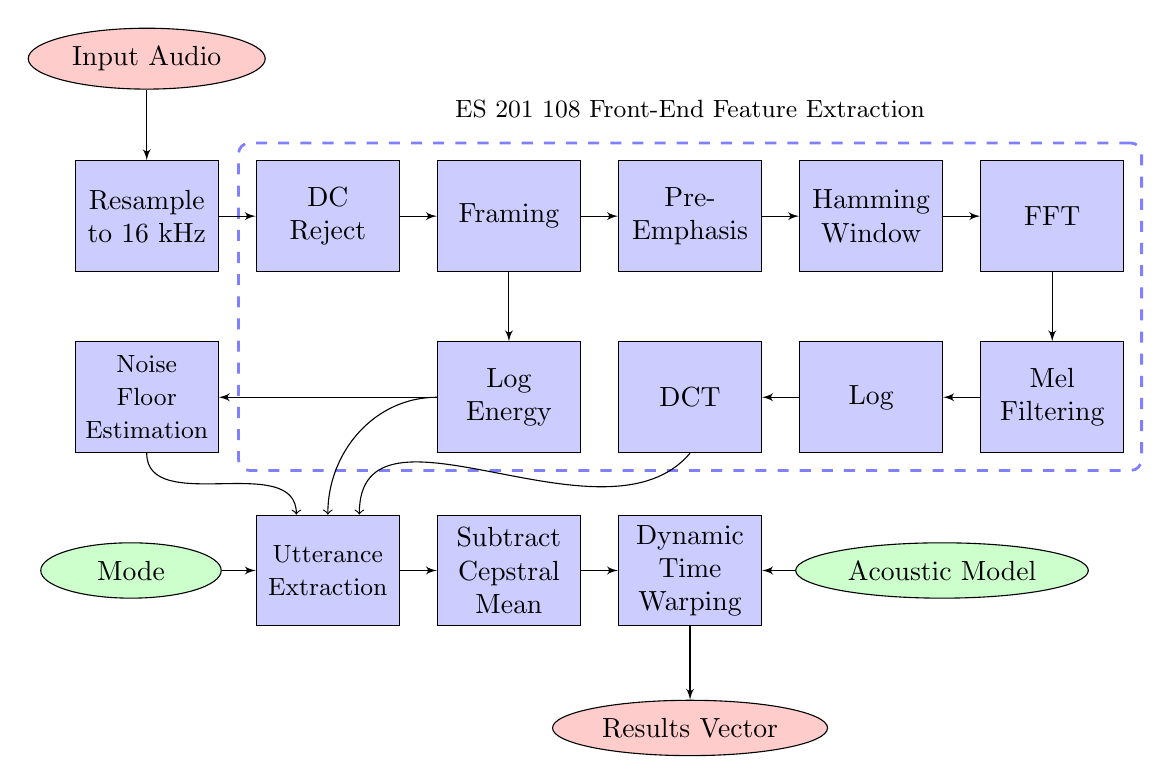
\begin{tikzpicture}[node distance=2cm, auto]
	\tikzset{blue dotted/.style={draw=blue!50!white, line width=1pt, dash pattern=on 4pt off 4pt, inner sep=2.2mm, rectangle, rounded corners}};
	\node [io] (audio) {Input Audio};
	\node [block, below of=audio, node distance=2cm] (resample) {Resample to 16 kHz};
	\node [block, right of=resample] (offset) {DC Reject};
	\node [block, right of=offset] (framing) {Framing};
	\node [block, right of=framing] (pe) {Pre-Emphasis};
	\node [block, right of=pe] (windowing) {Hamming Window};
	\node [block, right of=windowing] (fft) {FFT};
	\node [block, below of=fft] (mel) {Mel Filtering};
	\node [block, left of=mel] (log) {Log};
	\node [block, left of=log] (dct) {DCT};
	\node [block, below of=framing] (loge) {Log Energy};
	\node [block, below of=resample] (noisef) {\small{}Noise Floor Estimation};
	\node [blue dotted, fit=(offset) (loge) (mel)] (es201108) {};
	\node at (es201108.north) [above, inner sep=3mm] {\small ES 201 108 Front-End Feature Extraction};
	\node [block, below of=offset, node distance=4.5cm] (utter) {\small{}Utterance Extraction};
	\node [config, left of=utter, node distance=2.5cm] (mode) {\phantom{X}Mode\phantom{X}};
	\node [block, text width=4.5em, right of=utter] (cmn) {Subtract Cepstral Mean};
	\node [block, right of=cmn] (dtw) {Dynamic Time Warping};
	\node [config, right of=dtw, node distance=3.2cm] (model) {Acoustic Model};
	\node [io, below of=dtw, node distance=2cm] (output) {Results Vector};
	\path [line] (audio) -> (resample);
	\path [line] (resample) -> (offset);
	\path [line] (offset) -> (framing);
	\path [line] (framing) -> (pe);
	\path [line] (pe) -> (windowing);
	\path [line] (windowing) -> (fft);
	\path [line] (fft) -> (mel);
	\path [line] (mel) -> (log);
	\path [line] (log) -> (dct);
	\path [line] (framing) -> (loge);
	\path [line] (loge) -> (noisef);
	\path [line] (mode) -> (utter);
	\draw (noisef.south) edge[->,out=270,in=90] ([xshift=-4mm]utter.north);
	\draw (dct.south) edge[->,out=230,in=90] ([xshift=4mm]utter.north);
	\draw (loge.west) edge[->,out=180,in=90] ([xshift=0mm]utter.north);
	\path [line] (utter) -> (cmn);
	\path [line] (cmn) -> (dtw);
	\path [line] (dtw) -> (output);
	\path [line] (model) -> (dtw);
\end{tikzpicture}}
\end{center}
Each processing block in the above diagram is detailed below.

\subsection{Front End}
The front end is responsible for converting the raw audio input into a stream of comparatively low dimensional feature vectors.
This is the main dimensionality reduction step in the recognizer.
Specifically, ES 201 108 is implemented in TinySR, so a vector of 13 cepstral coefficients is generated every 10 ms from the input audio stream.
If the input is 44.1 kHz stereo audio, then this step reduces the dimensionality of the input by a factor of about 68. 

\subsubsection{Resampling}
The rest of the DSP chain is specifically tuned for 16 kHz mono audio, so all input audio is downmixed and resampled as necessary before further processing occurs.
This is consistent with the choices made in other recognizers, such as CMU Sphinx, and is also the highest sampling rate for which ES 201 108 feature extraction is defined.
There is good reason to believe that having a Nyquist frequency above 8 kHz is wasteful, as very little useful speech energy is present above such a cutoff.
Currently the resampling is achieved via linear interpolation for simplicity, which (while being a crummy resampling filter) is good enough.
You can play wih \texttt{playground/resample.py} to resample audio with the same linear interpolation filter, to hear what sorts of distortions it introduces.

\subsubsection{ES 201 108 Feature Extraction}
These steps are well described in \href{http://www.etsi.org/deliver/etsi_es/201100_201199/201108/01.01.02_60/es_201108v010102p.pdf}{the original spec}, but also briefly described here.
\newcommand{\linear}{{\small\color{red}(L)}}
Each step that is linear is marked with \linear.
\renewcommand{\labelenumi}{\textbf{\Roman{enumi}.}}%
\begin{enumerate}
\item \linear{} An LTI DC rejection filter is applied to the input audio.
\item \linear{} The audio is framed in a ``sliding window'' fashion, by producing a frame of 400 samples (25 ms) every 160 samples (10 ms).
This means that each frame overlaps the previous by 240 samples (15 ms).
All further steps apply to each frame individually.
\item The log of the sum of the squares of the samples is computed, and is the ``log energy'' $E$ for the frame. (Depicted as the center input to ``Utterance Extraction,'' and the input to ``Noise Floor Estimation.'')
\item \linear{} An LTI high-pass (pre-emphasis) filter is applied. The filter simply subtracts 97\% of each sample from the next.
\item \linear{} The frame is \href{http://en.wikipedia.org/wiki/Window_function#Hamming_window}{Hamming windowed}.
\item \linear{} The frame is zero padded with 112 zero samples, to extend it out to 512 samples.
\item \linear{} An FFT is applied to the extended frame, then the absolute value is taken, to produce 512 real samples.
As the input data is pure real, Hermitian symmetry is present in the FFT output.
Thus, after the absolute value is taken, regular symmetry is present in the results, meaning that FFT bin $n$ is equal to FFT bin $512 - n$.
Therefore, all but the first 257 FFT bins are ignored after the transform.
\item \linear{} Twenty three overlaping triangular filters are dotted against the resulting FFT bins, to produce 23 Mel amplitude coefficients.
\item The natural log of each Mel amplitude coefficient is taken, to produce a Mel energy coefficient.
\item \linear{} A DCT-inspired linear transform of these coefficients is taken, producing 13 Mel cepstral coefficients, $C_i$ for $0 \le i \le 12$. (Depicted as the rightmost input to ``Utterance Extraction.'')
\end{enumerate}

\subsubsection{Noise Floor Estimation}
In order to detect utterances TinySR looks for frames that exceed the background noise floor by a substantial amount.
Thus, a robust running estimate of the noise floor $\eta$ is required.
Intuitively, the energy of a frame can never be below the noise floor, so $\eta \le E$ seems a reasonable precept.
For each frame, $\eta$ is set to the minimum of $E$ and $0.999 \cdot \eta + 0.001 \cdot E$.
This results in a ``slow to rise, fast to fall'' estimator, that falls instantaneously if $E$ should dip below $\eta$, and otherwise rises to $E$ with a time constant of ten seconds.
(The resulting $\eta$ is depicted as the leftmost input to ``Utterance Extraction.'')

\subsubsection{Feature Vector Assembly}
After all of the above processing is complete, a feature vector consisting of the fifteen scalars $\eta$, $E$, and $C_0$ through $C_{12}$ is assembled, and stored in the \texttt{fv\_list} member variable of a TinySR context.

\subsection{Back End}
The back end's job is to take the dimensionally reduced stream of feature vectors, and actually perform recognition.
At this point, TinySR's operation is configured by the user.
If TinySR is operating in ``free running'' mode, then utterances are detected and picked out of the input stream.
This mode of operation is suitable for implementing a voice command interface, in which the user may speak a command at any time, but not all utterances are necessarily commands.
For example, an automotive application with commands like ``turn off/on AC.''

Alternatively, if TinySR is operating in ``one shot'' mode, then utterance detection is skipped, and the entire audio input is assumed to be a single utterance.
This is suitable for implementing an application in which each voice command is explicitly delimited, for example if the user holds a button while speaking, and releases it when done.

Regardless, the back end consists of a few steps.

\subsubsection{Utterance Extraction}
In one shot mode, this step is skipped.
However, in free running mode, utterance extraction is performed by looking at the log energies of successive frames.
Specifically, the log energy $E$ must exceed the noise floor $\eta$ by about 22 dB for at least 10 frames (100 ms), to begin an utterance.%
\footnote{This energy threshold parameter is tunable in \texttt{tinysr.c} as \texttt{UTTERANCE\_START\_ENERGY\_THRESHOLD}, in natural units, where one point corresponds to about 4.3 dB. Further, the start and stop number frame counts are tunable in the same place.}
Once $E$ fails to exceed $\eta$ by about 4 dB for another 10 frames the utterance is considered complete.
After the start and end points are determined, some extra frames are taken before the beginning of the utterance, and the last few frames of the utterance are dropped.

\subsubsection{Cepstral Mean Normalization}
After an utterance is extracted, the mean cepstral 13-vector is computed across the utterance, and subtracted out from each feature vector within the utterance.
Observe that cepstrum is a linear transform on the log of the Fourier transform of the underlying data.
Therefore, adding cepstra results in Fourier space multiplication, which is convolution in time domain.
Thus, by subtracting out the mean cepstrum, we are effectively deconvolving the source signal.
Therefore, convolving the source signal with any finite impulse response kernel that fits within the periodicity of a single frame's FFT causes no net effect on the post-mean-normalization cepstrum.

This is a fantastic result, as the effects of the transfer function of a microphone are almost certainly very closely approximated as convolution with a small FIR filter.
Although this step takes only ten lines of code, it makes TinySR robust against differences in audio setup and inter-speaker variations.

\subsubsection{Dynamic Time Warping}
Here we match up an utterance against an acoustic model.
A model consists of a time series of multivariate Gaussian distributions, representing a prior on the cepstrum expected to form a given word.
Each Gaussian is characterized by a 13 dimensional mean $\mu$ and a $13\times13$ covariance matrix $\Sigma$.
We will denote the log likelihood of a cepstral column vector $C$ matching a model $(\mu, \Sigma)$ by $P\left(C, (\mu, \Sigma)\right)$, as given by:
\begin{align*}
P\left(C, (\mu, \Sigma)\right) = - \frac12 \log | \Sigma | - \frac12 (C - \mu)^T \Sigma^{-1} (C - \mu)
\end{align*}

Thus, we have a way of matching a vector against a model.
We can therefore compute an overall log likelihood for a time series of cepstral feature vectors $C_i$ matching a model $(\mu_i, \Sigma_i)$ by computing $\sum_i P(C_i, (\mu_i, \Sigma_i))$.
However, this requires that the model be of exactly the same length as the input speech, and further that the speaker's utterance exactly lines up against the model.

To fix these issues, we perform dynamic time warping, which is consists of finding a minimum cost path through the matrix $A$ with $A_{ij} = P(C_i, (\mu_j, \Sigma_j))$.
The path may only make three kinds of moves:
\begin{enumerate}
\item Diagonally, from $(i, j)$ to $(i+1, j+1)$.
This corresponds to matching feature $i$ in the utterance directly against Gaussian $j$ in the model.
\item Horiztonally, from $(i, j)$ to $(i+1, j)$.
This corresponds to the speaker speaking slowing during frames $i$, and $i+1$, and them both being matched against model Gaussian $j$.
\item Vertically, from $(i, j)$ to $(i, j+1)$.
This corresponds to the speaker speaking quickly during frame $i$, and it being matched against both model Gaussians $j$ and $j+1$.
\end{enumerate}
Further, we demand that our path starts at $(i, j) = (1, 1)$, and that it ends at $(i, j) = (n, m)$, where there are $n$ frames in our utterance and $m$ frames (Gaussians) in our model.
This guarantees that the utterance's beginning matches up against the model's beginning, and the same for the end.

\section{Training}
To train a model for a given word, we need merely produce a series of Gaussian distributions characterizing the time dynamics of the cepstrum.
To do this, we start with an input corpus of one or more speakers saying the same word over and over, and choose an urtterance of median length.
Our initial model consists simply of the series of Guassians whose means are the cepstral vectors in the chosen utterance, and with identity covaraiance.

Next, we refine this model to convergence, by the following steps:
\begin{enumerate}
\item Line every word in our corpus up against our model using DTW.
\item Find all the cepstral feature vectors that were matched against frame $i$ in the model, and use these to estimate the next Gaussian for frame $i$ in our iterated model.
\item Repeat if the generated model is different from the previous model.
\end{enumerate}
In practice, this method tends to converge within five or six iterations, and is extremely stable to variations in some initial parameters.
For example, which word of median length selected hardly matters, and the identity covariance matrix can be replaced by almost anything else non-degenerate.
The only important dependence that is carried forwards from the initial model to the final model is the length, which cannot change throughout the refinement; thus, why we select a median length utterance to start with.

\subsection{Gaussian Fitting}
One step glossed over above is how we fit a Gaussian to a set of $N$ cepstral observation $C_i$ for $1 \le i \le N$.
Each observation $C_i$ is, as always, a 13 dimensional vector, describing the harmonic content of frame of time.
First, the sample mean is computed, $\mu = \sum_{i=1}^N C_i / N$.
Next, the sample covariance is computed, given by:
\begin{align*}
\Sigma = \frac1{N-1} \sum_{i=1}^N (C_i - \mu) (C_i - \mu)^T
\end{align*}
In short, $\mu$ is the expected value, and $\Sigma$ is the expected self-outer-product over the meanless data.

\end{document}
